\PassOptionsToPackage{unicode=true}{hyperref} % options for packages loaded elsewhere
\PassOptionsToPackage{hyphens}{url}
\documentclass[14pt,ignorenonframetext,compress]{beamer}
\IfFileExists{pgfpages.sty}{\usepackage{pgfpages}}{}
\setbeamertemplate{caption}[numbered]
\setbeamertemplate{caption label separator}{: }
\setbeamercolor{caption name}{fg=normal text.fg}
\beamertemplatenavigationsymbolsempty
\usepackage{lmodern}
\usepackage{amssymb,amsmath}
\usepackage{ifxetex,ifluatex}
\usepackage{fixltx2e} % provides \textsubscript
\ifnum 0\ifxetex 1\fi\ifluatex 1\fi=0 % if pdftex
  \usepackage[T1]{fontenc}
  \usepackage[utf8]{inputenc}
\else % if luatex or xelatex
  \ifxetex
    \usepackage{mathspec}
  \else
    \usepackage{fontspec}
\fi
\defaultfontfeatures{Ligatures=TeX,Scale=MatchLowercase}







\fi

  \usetheme[]{monash}

  \usecolortheme{monashwhite}


% A default size of 24 is set in beamerthememonash.sty

% Title page
\setbeamertemplate{title page}
{\placefig{-0.01}{-0.01}{width=1.01\paperwidth,height=1.01\paperheight}{titlepage}
\begin{textblock}{7.5}(1,2.8)\usebeamerfont{title}
{\color{white}\raggedright\par\inserttitle}
\end{textblock}
\begin{textblock}{7.5}(1,7)
{\color{white}\raggedright{\insertauthor}\mbox{}\\[0.2cm]
\insertdate}
\end{textblock}}




% use upquote if available, for straight quotes in verbatim environments
\IfFileExists{upquote.sty}{\usepackage{upquote}}{}
% use microtype if available
\IfFileExists{microtype.sty}{%
  \usepackage{microtype}
  \UseMicrotypeSet[protrusion]{basicmath} % disable protrusion for tt fonts
}{}


\newif\ifbibliography


\hypersetup{
      pdftitle={A framework for detecting anomalies in water-quality variables},
        pdfauthor={Puwasala Gamakumara},
          pdfborder={0 0 0},
    breaklinks=true}
%\urlstyle{same}  % Use monospace font for urls






  \usepackage{graphicx,grffile}
  \makeatletter
  \def\maxwidth{\ifdim\Gin@nat@width>\linewidth\linewidth\else\Gin@nat@width\fi}
  \def\maxheight{\ifdim\Gin@nat@height>\textheight0.8\textheight\else\Gin@nat@height\fi}
  \makeatother
  % Scale images if necessary, so that they will not overflow the page
  % margins by default, and it is still possible to overwrite the defaults
  % using explicit options in \includegraphics[width, height, ...]{}
  \setkeys{Gin}{width=\maxwidth,height=\maxheight,keepaspectratio}

% Prevent slide breaks in the middle of a paragraph:
\widowpenalties 1 10000
\raggedbottom

  \AtBeginPart{
    \let\insertpartnumber\relax
    \let\partname\relax
    \frame{\partpage}
  }
  \AtBeginSection{
    \ifbibliography
    \else
      \let\insertsectionnumber\relax
      \let\sectionname\relax
      \frame{\sectionpage}
    \fi
  }
  \AtBeginSubsection{
    \let\insertsubsectionnumber\relax
    \let\subsectionname\relax
    \frame{\subsectionpage}
  }



\setlength{\parindent}{0pt}
\setlength{\parskip}{6pt plus 2pt minus 1pt}
\setlength{\emergencystretch}{3em}  % prevent overfull lines
\providecommand{\tightlist}{%
  \setlength{\itemsep}{0pt}\setlength{\parskip}{0pt}}

  \setcounter{secnumdepth}{0}


%% Monash overrides
\AtBeginSection[]{
   \frame<beamer>{
   \frametitle{Outline}\vspace*{0.2cm}
   
   \tableofcontents[currentsection,hideallsubsections]
  }}

% Redefine shaded environment if it exists (to ensure text is black)
\ifcsname Shaded\endcsname
  \definecolor{shadecolor}{RGB}{225,225,225}
  \renewenvironment{Shaded}{\color{black}\begin{snugshade}\color{black}}{\end{snugshade}}
\fi
%%

  % Colors
  \setbeamercolor{description item}{fg=Orange}
  \definecolor{MonashBlue}{RGB}{73,129,175}
  % Colors
  \definecolor{DarkBrown}{RGB}{80,70,60}
  \setbeamercolor{description item}{fg=Orange}
  \setbeamercolor{block title alerted}{fg=white,bg=DarkBrown}
  \setbeamercolor{block title}{fg=white,bg=DarkBrown}
  \setbeamercolor{frametitle}{bg=DarkBrown,fg=white}

  % Packages
  \usepackage{amsmath, nccmath, graphicx}
  \usepackage{bm}
  \usepackage{mathpazo}
  \usepackage{booktabs}
  \usepackage{fontawesome}


  % Monash title page
  \setbeamertemplate{title page}
  {\placefig{-0.01}{-0.01}{width=1.01\paperwidth,height=1.01\paperheight}{Title-page.jpg}
  \begin{textblock}{10.5}(0.5,2.8)\usebeamerfont{title} %2.8
  {\color{white}\raggedleft\par\inserttitle}
  \end{textblock}
  \begin{textblock}{5.5}(0.5,7)
  {\color{white}\raggedleft\par\insertauthor\mbox{}}
  \end{textblock}
  \begin{textblock}{5.5}(0.5,7.8)
  {\color{white}\raggedleft\par\insertdate\mbox{}}
  \end{textblock}}



  \title[]{A framework for detecting anomalies in water-quality
variables}

  \subtitle{Importance of having multiple sensors close to each other}

  \author[
        Puwasala Gamakumara
    ]{Puwasala Gamakumara}


\date[
      ARCLP Workshop
  ]{
      ARCLP Workshop
        }

\begin{document}

% Hide progress bar and footline on titlepage
  \begin{frame}[plain]
  \titlepage
  \end{frame}


   \frame<beamer>{
   \frametitle{Outline}\vspace*{0.2cm}
   
   \tableofcontents[hideallsubsections]
  }

\hypertarget{introduction}{%
\section{Introduction}\label{introduction}}

\begin{frame}{Water-quality monitoring in river networks}
\protect\hypertarget{water-quality-monitoring-in-river-networks}{}
\begin{itemize}
\item
  Low-cost in-situ sensors
\item
  Produce high-frequency data
\item
  Prone to errors due to miscalibration, biofouling, battery and
  technical errors
\end{itemize}

\begin{block}{Objective}
\protect\hypertarget{objective}{}
\begin{itemize}
\tightlist
\item
  Developing statistical tools to detect anomalies in water-quality
  variables measured by in-situ sensors
\item
  Extend to utilising information from multiple sensors
\end{itemize}
\end{block}
\end{frame}

\hypertarget{framework}{%
\section{Framework}\label{framework}}

\begin{frame}{Anomaly detection framework}
\protect\hypertarget{anomaly-detection-framework}{}
\emph{An anomaly is an observation that has an unexpectedly low
conditional density}

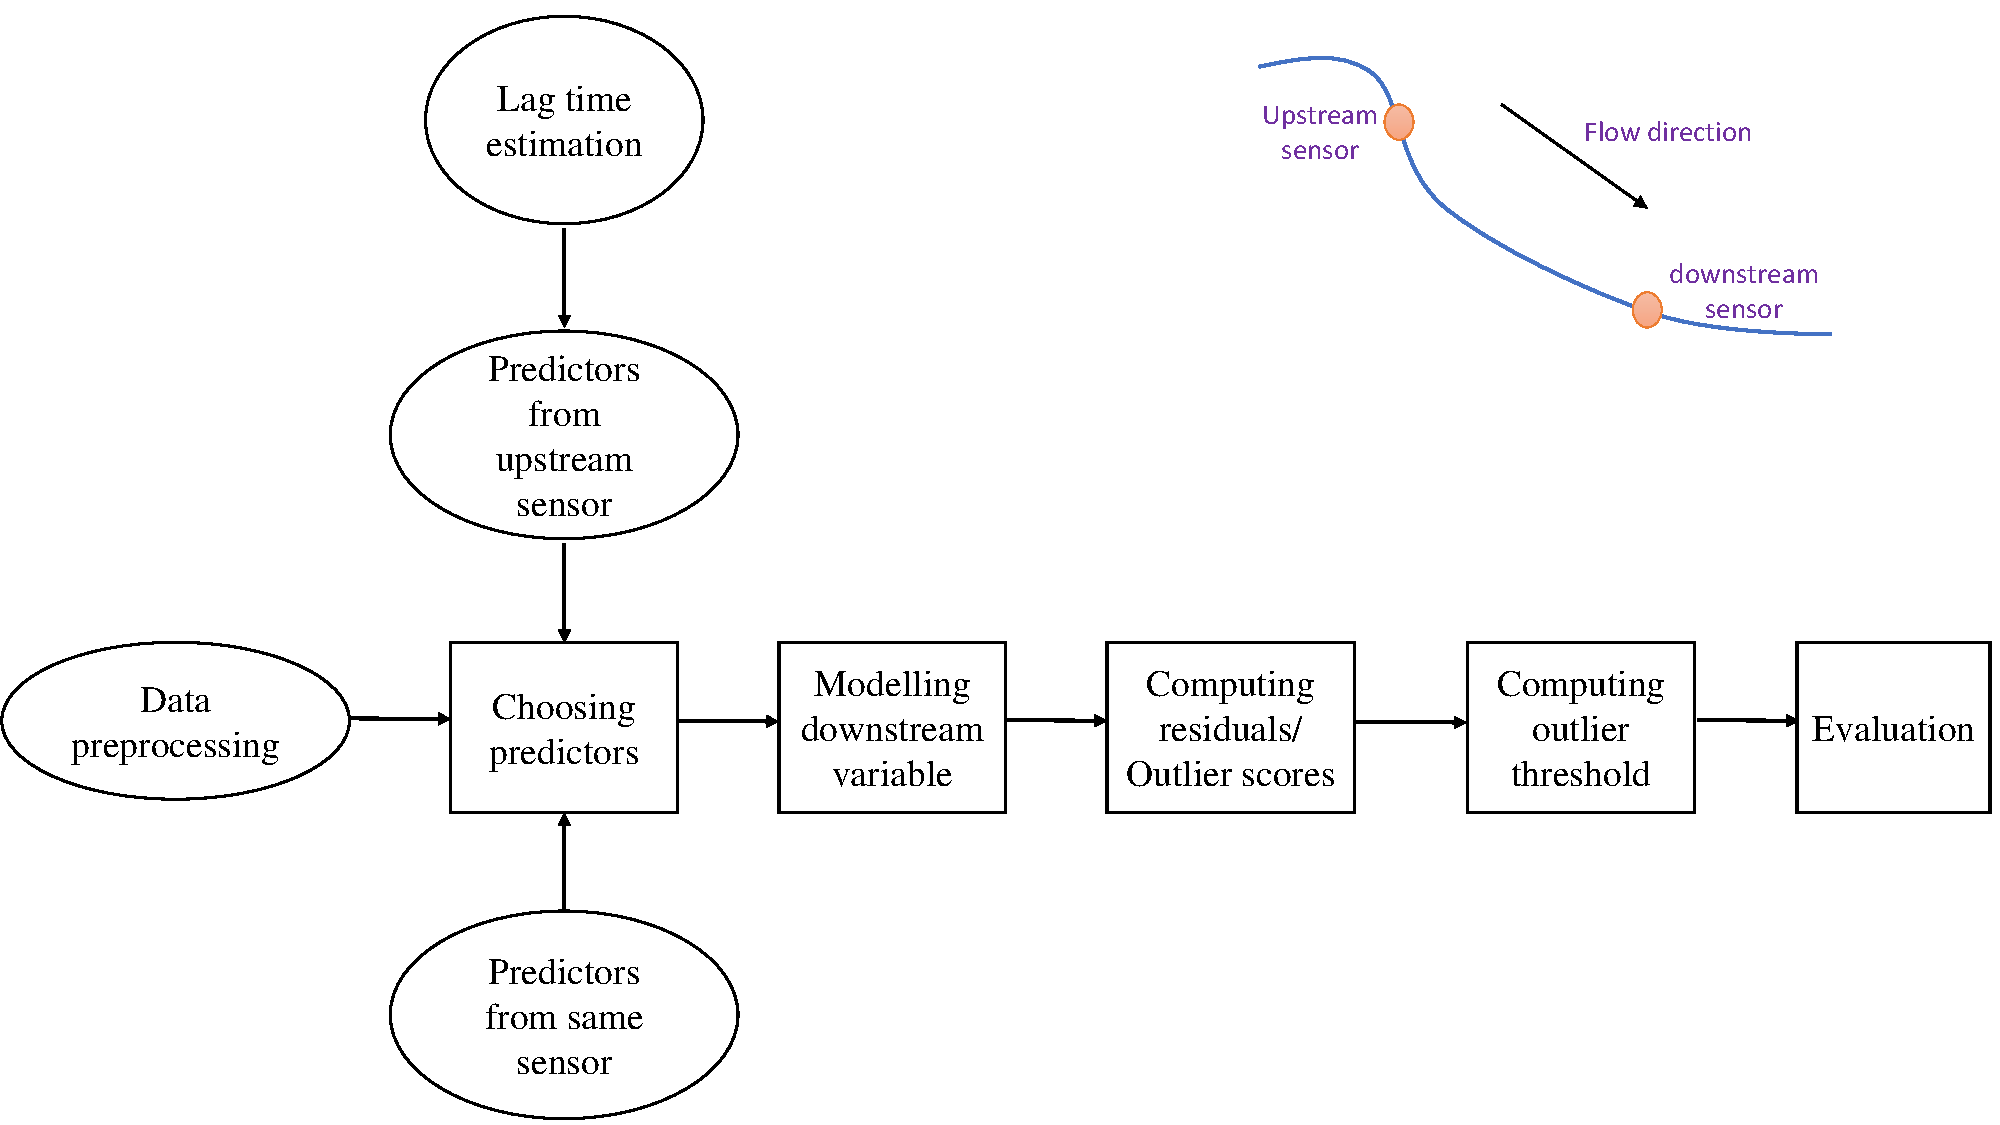
\includegraphics{C:/Puwasala/ARCLP-workshop/presentation/plots/Framework.pdf}
\end{frame}

\hypertarget{data}{%
\section{Data}\label{data}}

\begin{frame}{Pringle Creek - Texas, USA}
\protect\hypertarget{pringle-creek---texas-usa}{}
\begin{figure}
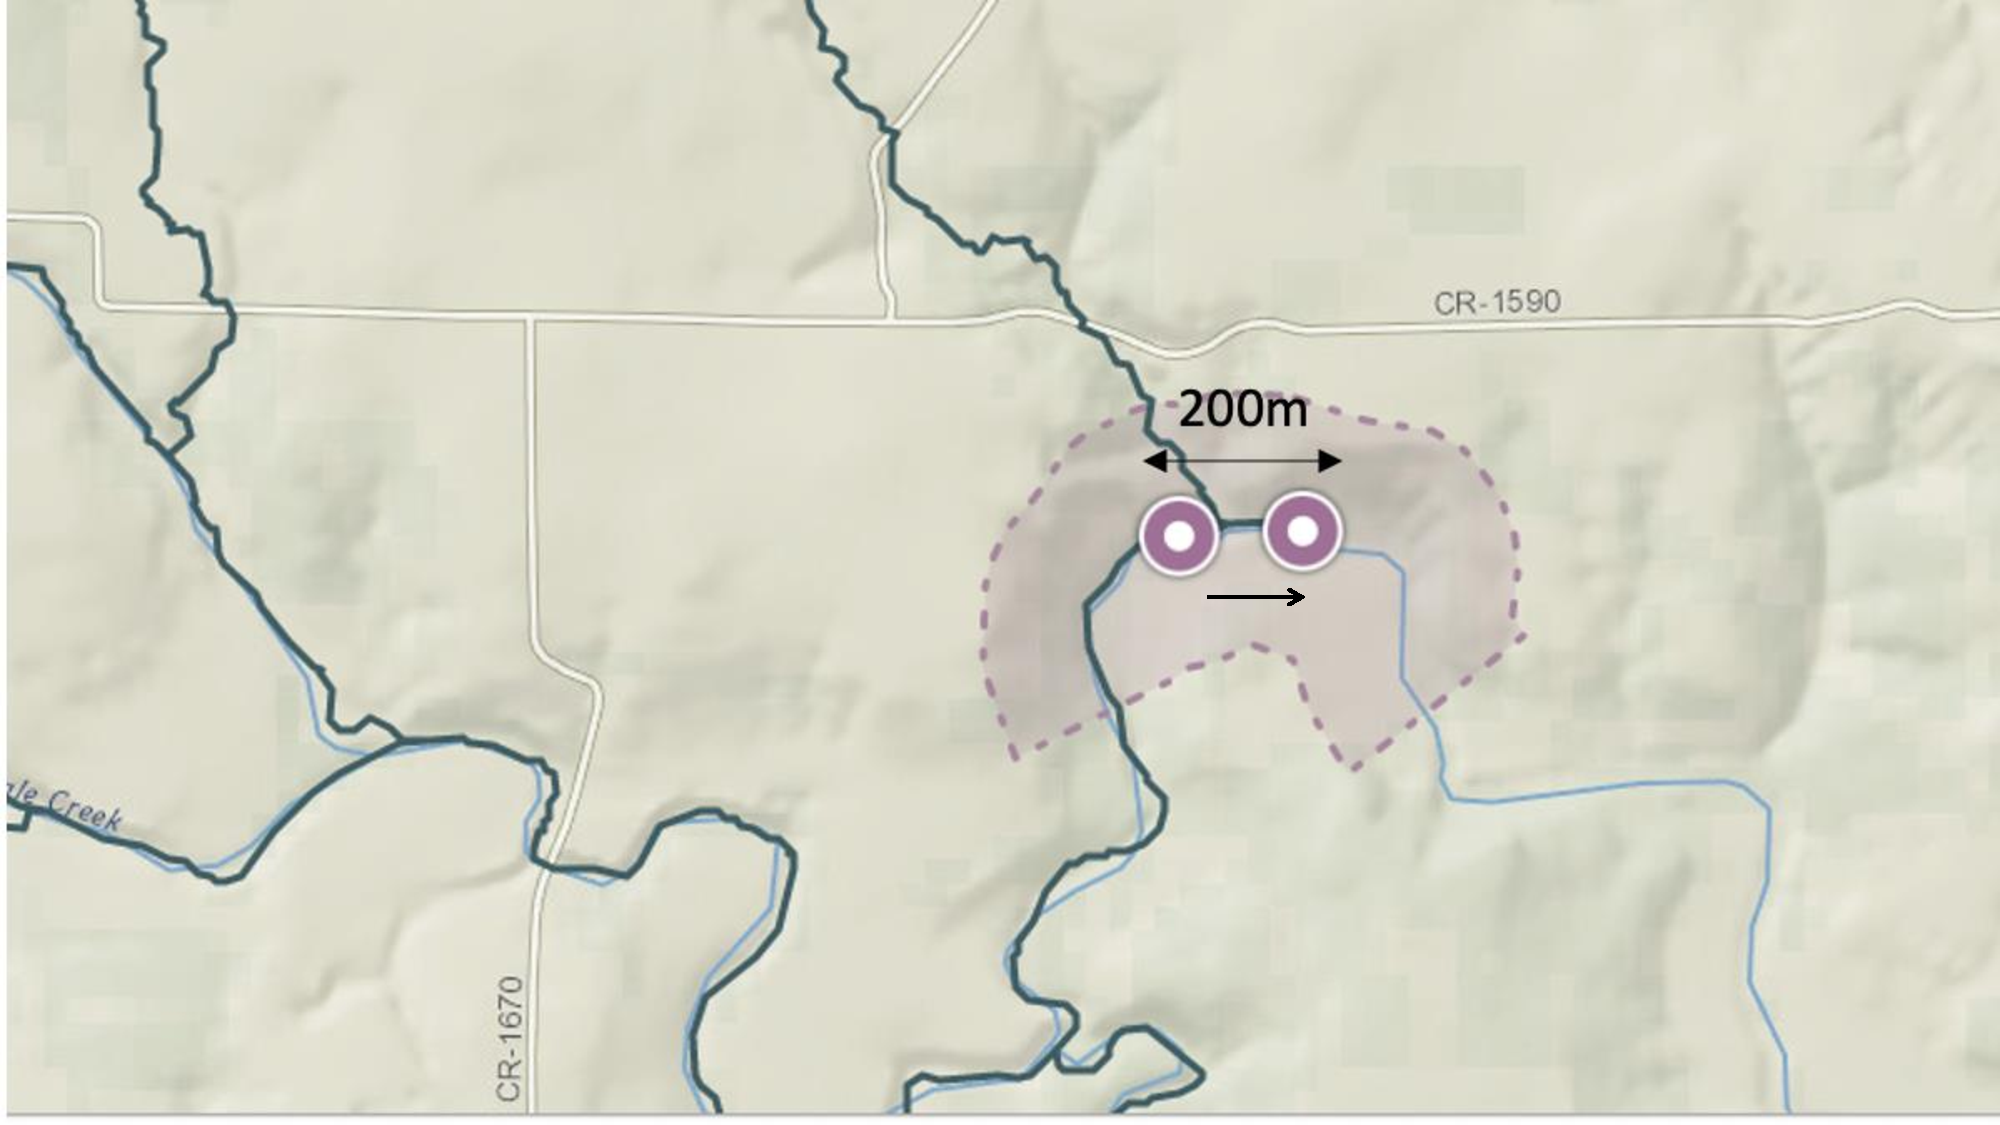
\includegraphics[width=1\linewidth]{plots/Pringle-creek-map} \caption{image courtesy neonscience.org}\label{fig:pringle-creek-map}
\end{figure}
\end{frame}

\begin{frame}{Data}
\protect\hypertarget{data-1}{}
\begin{itemize}
\item
  \textbf{Variables} - Turbidity, Conductivity, Dissolved oxygen, Level
  and Temperature
\item
  \textbf{Time span} - 01-10-2019 to 31-12-2019
\item
  \textbf{Frequency} - 5 minute intervals
\item
  {[}\url{https://data.neonscience.org/data-products}{]}
\end{itemize}
\end{frame}

\begin{frame}{Time plots}
\protect\hypertarget{time-plots}{}
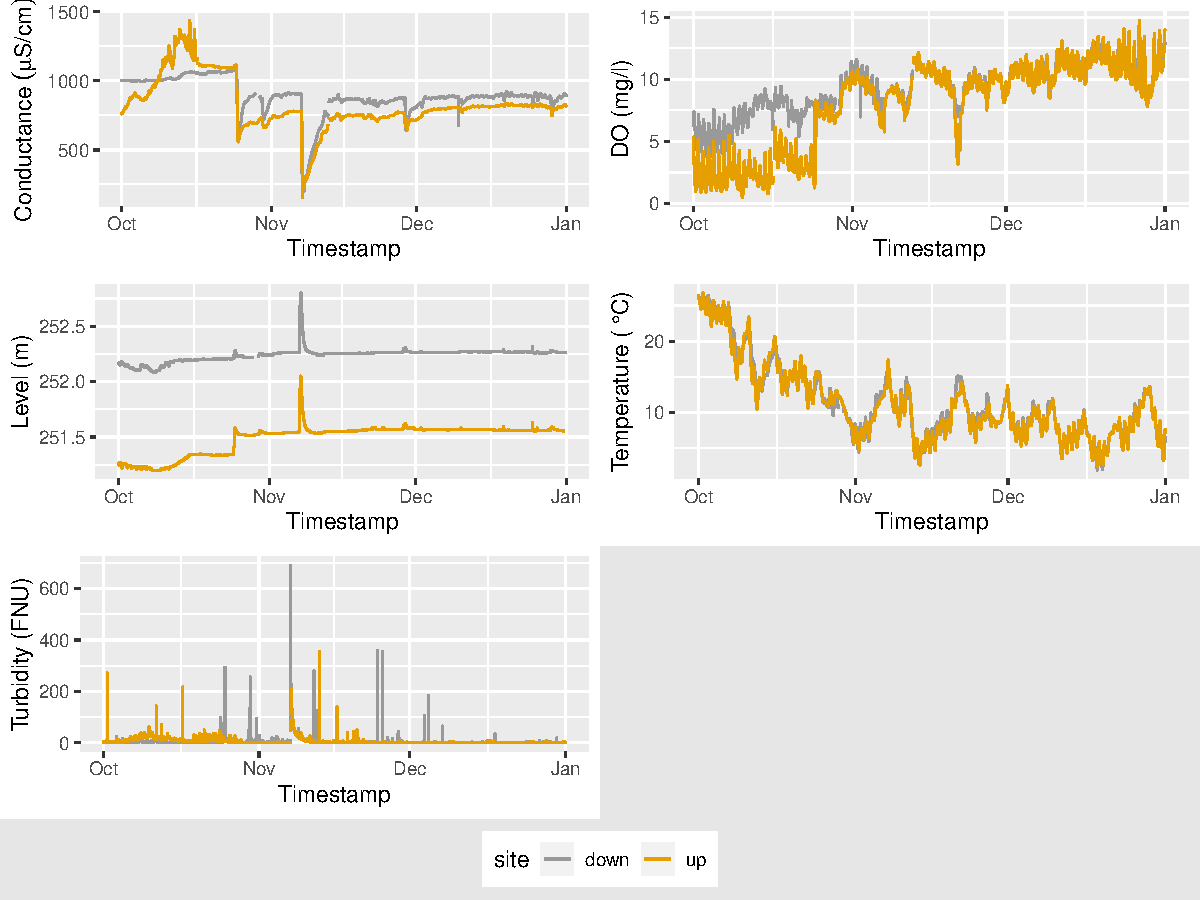
\includegraphics[width=1\linewidth]{slides_files/figure-beamer/tsplots-1}
\end{frame}

\begin{frame}
\begin{block}{Turbidity downstream vs other downstream variables}
\protect\hypertarget{turbidity-downstream-vs-other-downstream-variables}{}
\includegraphics[width=1\linewidth]{slides_files/figure-beamer/turbdown-down-plot-1}
\end{block}
\end{frame}

\begin{frame}
\begin{block}{Turbidity downstream vs other upstream variables}
\protect\hypertarget{turbidity-downstream-vs-other-upstream-variables}{}
\includegraphics[width=1\linewidth]{slides_files/figure-beamer/turbdown-up-plot-1}
\end{block}
\end{frame}

\hypertarget{modeling}{%
\section{Modeling}\label{modeling}}

\begin{frame}{Modeling downstream turbidity}
\protect\hypertarget{modeling-downstream-turbidity}{}
\small

\begin{equation*}\label{eq:gam_main}
turbidity\_down_t = \phi_0 + \sum_{i=1}^pg_i(z_{i,t_l}) + \sum_{j=1}^qh_j(turbidity\_down_{t-j}) + \varepsilon_t
\end{equation*}

\begin{block}{Choices for \(z_{i,t_l}\)}
\protect\hypertarget{choices-for-z_it_l}{}
\begin{table}
\centering\begingroup\fontsize{10}{12}\selectfont

\resizebox{\linewidth}{!}{
\begin{tabular}[t]{ll}
\toprule
Model & Predictors\\
\midrule
GAM-down & other downstream variables\\
GAM-down-AR & other downstream variables + lagged responses\\
GAM-up & upstream variables\\
GAM-up-AR & upstream variables + lagged responses\\
GAM-up-down & upstream variables + downstream variables\\
\bottomrule
\end{tabular}}
\endgroup{}
\end{table}
\end{block}
\end{frame}

\begin{frame}{Lag time estimation}
\protect\hypertarget{lag-time-estimation}{}
\begin{itemize}
\item
  Assume the lag time between two sensor locations depends on the
  upstream river behavior
\item
  Use \emph{conditional cross-correlations} to estimate the lag time
\item
  let \(x_t:\) Turbidity upstream, \(y_t:\) Turbidity downstream and
  \(\bm{z}_t:\) \{level upstream, temperature upstream\}
\item
  \(x^*_t = \frac{x_t - \text{E}[x_t|\bm{z}_t]}{\sqrt{\text{V}[x_t|\bm{z}_t]}}\)
  and
  \(y^*_t = \frac{y_t - \text{E}[y_t|\bm{z}_t]}{\sqrt{\text{V}[y_t|\bm{z}_t]}}\)
\end{itemize}
\end{frame}

\begin{frame}
\begin{block}{Conditional cross-correlation}
\protect\hypertarget{conditional-cross-correlation}{}
\[
r_k(\bm{z}_t) = \text{E}[x_t^*y^*_{t+k}|\bm{z}_t] \quad \text{for} \quad k = 1,2,...
\]

\begin{itemize}
\item
  To estimate \(r_k(\bm{z}_t)\) we fit the following GAMs
\item
  Let
  \(x_t^*y^*_{t+k}|\bm{z}_t \sim \text{N}(r_k(\bm{z}_t), \sigma_r^2)\),
\end{itemize}

\[
g(r_k(\bm{z}_t)) = \gamma_0 + \sum_{i=1}^p h_i(z_{i,t}) + \varepsilon_t
\]

\[
\hat{r}_k(\bm{z}_t) = g^{-1}( \hat{\gamma}_0 + \sum_{i=1}^p \hat{h}_i(z_{i,t}))
\]
\end{block}

\begin{block}{Estimating time delay}
\protect\hypertarget{estimating-time-delay}{}
\[
\hat{d}_{t}(\bm{z}_t) = \underset{k}{\operatorname{argmax}}\quad \hat{r}_{k}(\bm{z}_t)
\]
\end{block}
\end{frame}

\begin{frame}{Conditional cross-correlation and lag time estimation}
\protect\hypertarget{conditional-cross-correlation-and-lag-time-estimation}{}
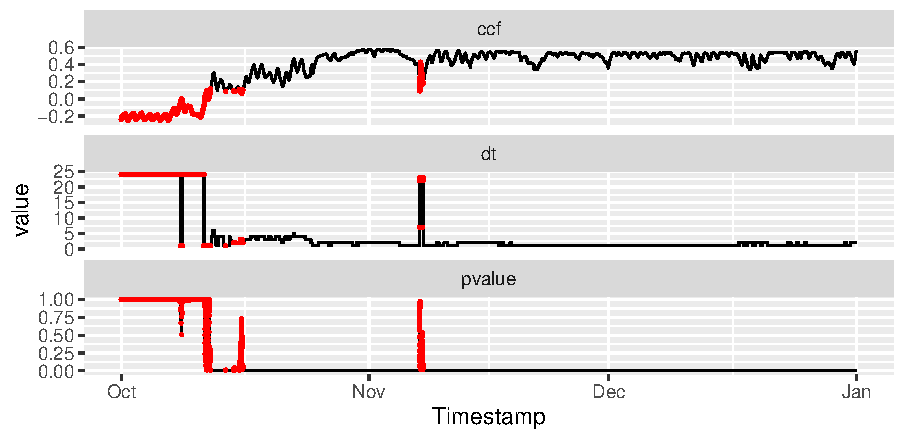
\includegraphics[width=1\linewidth]{plots/plot_ccf_dt_pval}
\end{frame}

\begin{frame}
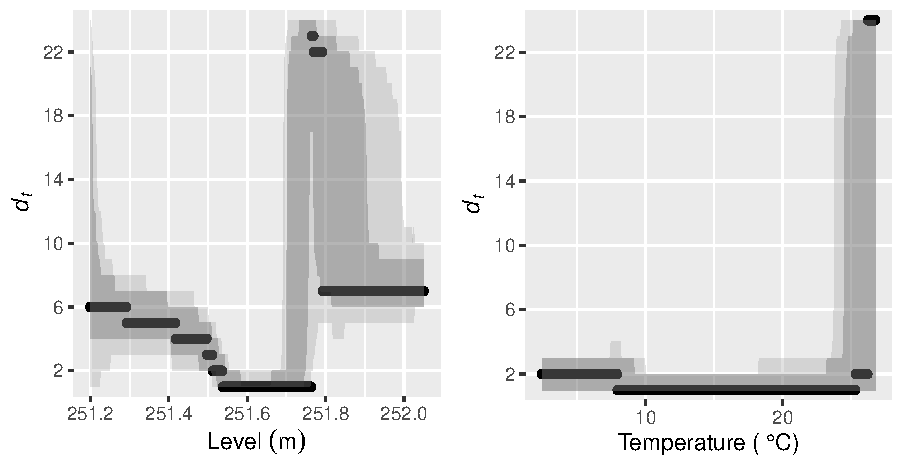
\includegraphics[width=1\linewidth]{plots/vis_dt}
\end{frame}

\hypertarget{outlier-detection-based-on-extreme-value-theory}{%
\section{Outlier detection based on Extreme value
theory}\label{outlier-detection-based-on-extreme-value-theory}}

\begin{frame}{Outlier detection using Peak over Threshold method}
\protect\hypertarget{outlier-detection-using-peak-over-threshold-method}{}
\includegraphics[width=1\linewidth]{slides_files/figure-beamer/classification-all-models-1}
\end{frame}

\hypertarget{evaluation}{%
\section{Evaluation}\label{evaluation}}

\begin{frame}{Performance Evaluation}
\protect\hypertarget{performance-evaluation}{}
\begin{table}
\centering\begingroup\fontsize{7}{9}\selectfont

\resizebox{\linewidth}{!}{
\begin{tabular}[t]{lrrrrr}
\toprule
method & TP & TN & FP & FN & OP\\
\midrule
GAM-down-AR & 15 & 25948 & 39 & 0 & 0.9977\\
GAM-up-down & 14 & 25916 & 14 & 1 & 0.9652\\
GAM-up-AR & 14 & 25837 & 21 & 1 & 0.9651\\
GAM-up & 10 & 25920 & 10 & 5 & 0.7996\\
stray(p=0.5, k=1) & 9 & 26007 & 5 & 6 & 0.7497\\
stray(p=0.5, k=5) & 6 & 26011 & 1 & 9 & 0.5711\\
stray(p=0.75, k=5) & 6 & 26011 & 1 & 9 & 0.5711\\
GAM-down & 5 & 26012 & 0 & 10 & 0.4996\\
stray(p=0.75, k=1) & 15 & 9835 & 16177 & 0 & -0.0728\\
\bottomrule
\end{tabular}}
\endgroup{}
\end{table}
\end{frame}

\hypertarget{conclusion}{%
\section{Conclusion}\label{conclusion}}

\begin{frame}{Conclusions}
\protect\hypertarget{conclusions}{}
\begin{itemize}
\item
  A new framework to detect technical anomalies
\item
  Uses temporal correlation between the water-quality variables to
  detect anomalies
\item
  Utilising information from the nearby sensors improves the performance
  of the algorithm
\item
  Place low-cost sensors close together
\end{itemize}
\end{frame}

\begin{frame}
\begin{center}
\Huge \emph{Thank You!}
\end{center}

\begin{block}{}
Slides: \textcolor{blue}{\url{https://github.com/PuwasalaG/ARCLP-workshop/tree/main/presentation}}
\vspace*{1cm}

\href{https://github.com/PuwasalaG}{\faicon{github}  @PuwasalaG}

\href{mailto:puwasala.gamakumara@gmail.com}{\faicon{envelope}  puwasala.gamakumara@gmail.com}
\end{block}
\end{frame}




\end{document}
